\documentclass[10pt]{beamer}

\usepackage{appendixnumberbeamer}

\usepackage{booktabs}
\usepackage[scale=2]{ccicons}

\usepackage{pgfplots}
\usepgfplotslibrary{dateplot}

\usepackage{xspace}
\usepackage{../theme_style}
\setbeameroption{show notes on second screen}

\title[Positioning and location awareness]{Exam question 4 - Positioning and location awareness}
\subtitle{Distributed and Pervasive Systems}
\date{June 03, 2022}
\author[M.H. Kristensen]{Morten Haahr Kristensen}
\def\studentid{201807664}
\institute{Department of Electrical and Computer Engineering - Aarhus University}
% Logo only on title page
\titlegraphic{
    
\includegraphics[width=12cm]{figs/aulogo_big.png}
}
\begin{document}

\maketitle

\begin{frame}{Outline}
  \setbeamertemplate{section in toc}[sections numbered]
  \tableofcontents[hideallsubsections]
\end{frame}

\section{Motivation}

\begin{frame}{Motivation}
  \begin{alertblock}{Distributed System definition \cite{vansteenDistributedSystems2018}}
    A distributed system is a collection of autonomous computing elements that \textbf{appears} to its users as \textbf{a single coherent system}.
  \end{alertblock}
  \begin{itemize}
    \item Position and location is often central in distributed and pervasive systems.
    \item Principles learned in position and location can be applied in other course-relevant areas.
  \end{itemize}
\end{frame}

\section{Location and Positioning}

\begin{frame}
  \frametitle{Location vs. Position}

  Position:
  \vspace*{-0.7em}
  \begin{itemize}
    \item Coordinates
    \item Typically World Geodetic System (WGS)
  \end{itemize}

  Location:
  \vspace*{-0.7em}
  \begin{itemize}
    \item Qualitative description of a position
    \item E.g ''Storcenter Nord'' or ''Randersvej 122''
    \item Generated through \textbf{location services}
  \end{itemize}

  Location based service:
  \vspace*{-0.7em}
  \begin{itemize}
    \item Services based on the user's device's geographical location
    \item E.g. running app Endomondo
  \end{itemize}

\end{frame}

\begin{frame}
  \frametitle{Location based services}
  \LARGE

  TL;DR: It is easy to track people's location and companies are abusing it. 

  \scriptsize
  - a.k.a. Geoslavery
\end{frame}

\section{Absolute positioning}

\begin{frame}
  \frametitle{Overview}
  \tikzmark{triangulation_start}Triangulation\tikzmark{triangulation_end}
  \begin{itemize}
    \item Angles relative to beacons
    \item Position and orientation
  \end{itemize}

  Trilateration
  \begin{itemize}
    \item Distance relative to beacons
    \item Position only
  \end{itemize}
  
  \begin{tikzpicture}[remember picture,overlay]
    \node<2>[draw,line width=1pt,red,circle,ellipse,inner ysep=15pt, fit={(pic cs:triangulation_start) (pic cs:triangulation_end)}] {};
  \end{tikzpicture}
  \note{
    In regards to absolute positioning, there are generally two methods to use.\\
    Triangulation: Here we use our device's angle relative to the beacons to draw circles. We typically use three beacons to draw three circles and then we can determine the position and orientation based on where the circles intersect.\\
    Trilateration: Here we use the distance to the beacons to try and estimate the position. With two beacons we can narrow it down to two possible positions and with three we can find a single position.\\
    I will be focusing on triangulation as it seems to be more widely used. The ToTal\cite{pierlotNewThreeObject2014} article mentioned that there were many available angle sensors and that it was considered more accurate, robust and flexible. It also has the obvious benefit of providing orientation.
  }
\end{frame}

\begin{frame}
  \frametitle{Three object Triangulation algorithm - ToTal}
  Author's motivation:
  \begin{itemize}
    \item Limitations of other algorithms
    \note[item]{
      Other triangulation algorithms had limitations in beacon ordering, and blind spots or were computationally inefficient. I.e. have to solve equations of a quadratic system instead of a linear system.
    }
    \item Complexity of other algorithms
    \note[item]{
      The authors acknowledged that other algorithms with similar performance exist but they come with a cost of increased complexity. (Note this is the complexity of implementation and not software complexities)
    }
  \end{itemize}
\end{frame}


\begin{frame}
  \frametitle{ToTal - Power Center}
  \begin{figure}
    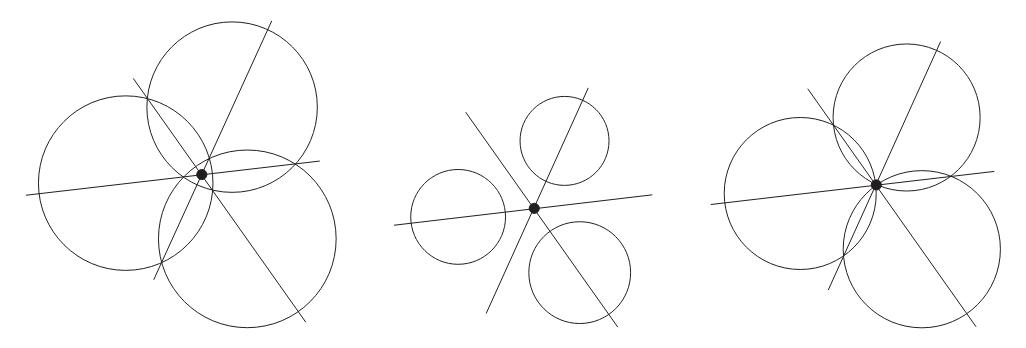
\includegraphics[width=\textwidth]{figs/total_power_center.png}
    \caption{Power center in three circles \cite{pierlotNewThreeObject2014}}
  \end{figure}
  \note{
    One thing that might need to be addressed is how the position is determined with noisy (real) sensors. One of the benefits of ToTal is that you will always get a result.\\
    In the ideal case, our measurements would always lead to a scenario like the right figure. The circles intersect perfectly on top of each other and narrow it down to a single point.\\
    When the data is noisy we can get cases like the middle and left figures. In the middle the circles never intersect and on the left, they overlap. \\ 
    To estimate the position based on this, the algorithm uses \textbf{power centers}. From each circle, they draw a line that intersects with the middle of the circle. This will bring three \textbf{power lines} where the point where they intersect defines the \textbf{power center} and it is our estimation of the position of the robot.\\
    Definition of \textbf{power center}: The power center of three circles is the unique point of equal power with respect to these circles.
  }

\end{frame}

\begin{frame}
  \frametitle{ToTal - Ambiguity removal}
  \begin{figure}
    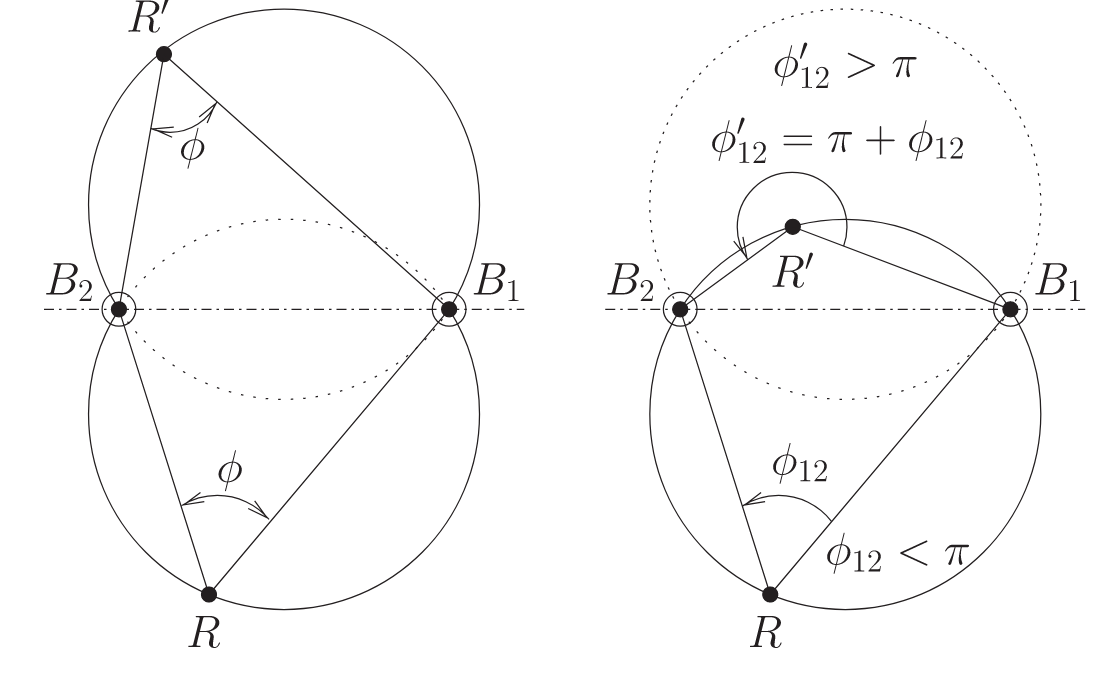
\includegraphics[width=\textwidth]{figs/total_phase_one.png}
    \caption{ToTal - Ambiguity removal \cite{pierlotNewThreeObject2014}}
  \end{figure}
  \note{
    This figure illustrates how ToTal handles ambiguity removal.\\
    The figure on the left is illustrating the necessity of removing ambiguity. If we don't do it then the position of the robot could be interpreted with the symmetry like on the left figure.\\
    We remove the locus ambiguity by the convention of always measuring angles counter-clockwise and by calculating the angles $\phi_{12} = \phi_2 - \phi_1$. This makes it so that the angle $\phi_{12}$ on the lower circle is always less than $\pi$ and the angle $\phi_{12}'$ upper circle is greater than $\pi$.\\
    When I first saw this figure I was a bit confused. If we know the position of the robot based on R, then why don't we just stop there? The figure is a bit misleading on this point. When we only use two beacons the robot's position can be anywhere on the circle. 
  }

\end{frame}

\begin{frame}
  \frametitle{ToTal - Geometric overview}
  \begin{figure}
    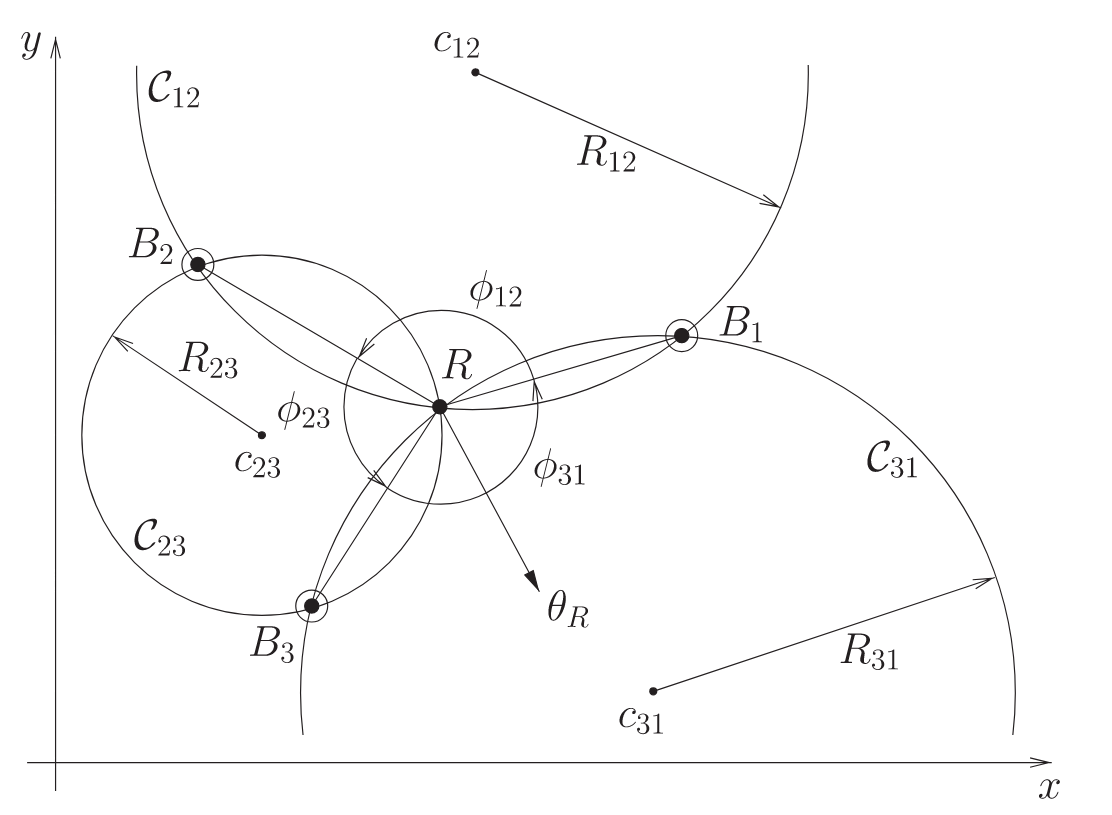
\includegraphics[width=0.8\textwidth]{figs/total_phase_two.png}
    \caption{ToTal - Triangulation setup \cite{pierlotNewThreeObject2014}}
  \end{figure}
  \note{
    Based on the angles to the beacons, we draw all the circles and calculate their parameters.\\
    We can see e.g. circle 31 $\mathcal{C}_{31}$ that is defined as the circle from beacon 3 to beacon 1. It has the angle $\phi_{31}$, center and radius. \\ 
    All the angles are measured with reference to the robot's heading orientation which is $\theta_R$.\\
    The article doesn't actually mention this but I assume this is known natively through the robot's sensor.
  }
\end{frame}

\begin{frame}
  \frametitle{ToTal - Algorithm I}
  \begin{figure}
    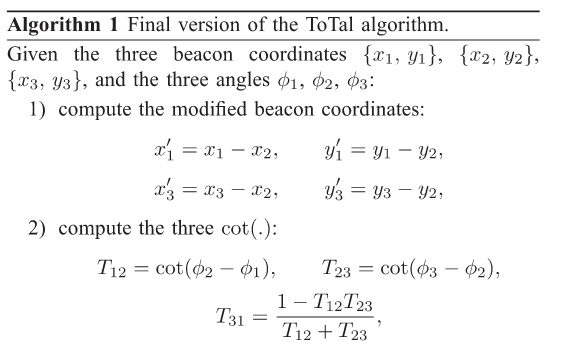
\includegraphics[width=0.7\textwidth]{figs/total_algorithm_1.png}
  \end{figure}
  \note{
    The algorithm uses the beacon positions relative to one of the beacons. (In the example beacon 2 is chosen). In the figure, they chose beacon 2 as the origin.\\
    Step one: Calculate the relative positions of the beacon coordinates.\\
    Step two: Intermediate results used in step 3. The last cotangent is calculated by referring to the other two cotangents as this is more computationally efficient.\\
  }
\end{frame}

\begin{frame}
  \frametitle{ToTal - Algorithm II}
  \begin{figure}
    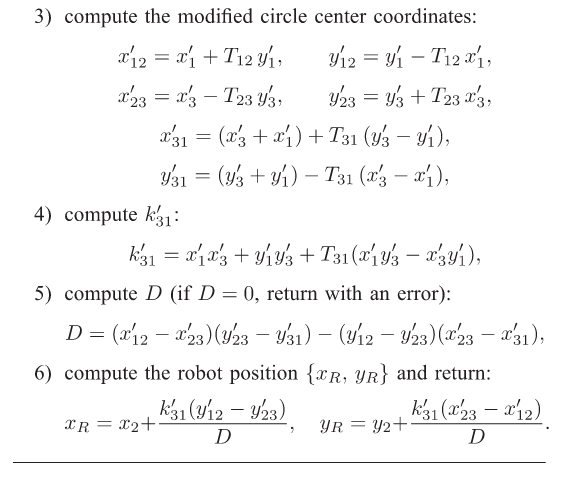
\includegraphics[width=0.7\textwidth]{figs/total_algorithm_2.png}
  \end{figure}
  \begin{equation*}
    k_{ij} = \frac{x_{ij}^2 + y_{ij}^2 - R_{ij}^2}{2}
  \end{equation*}
  \note{\footnotesize
    Step three: We calculate the coordinates of the circle center for each circle.\\
    Step four: The k-values are intermediate values that are used for calculating the power lines. They relate to the coordinates of the circle and its radius as seen in the formula. In this algorithm, it is only necessary to calculate a single one of them.\\
    Step five: The D-value is also used for the power lines where D stands for the denominator. During this step, we also need to check if it is zero to avoid dividing by zero in the next step. They write ''return an error'' but in reality, they have made a special case for handling these scenarios.\\
    My intuition tells me that this scenario might be entirely avoidable by the placement of the beacons. $D = 0$ when the circles are collinear which, to my understanding, means that they are in line. By having the beacons placed in a triangular shape this should not be possible. However, I would have to experiment more with this idea to be certain. It also makes sense that this is considered as it is a general algorithm.\\
    Step six: In the final step we calculate the robot's position.
  }
\end{frame}

\section{Relative positioning}

\begin{frame}
  \frametitle{Overview}
  Dead reckoning:
  \begin{itemize}
    \item Method for estimating current position
    \item Deduce position based on velocity, angle, time, and previously determined position.
  \end{itemize}
\end{frame}

\begin{frame}
  \frametitle{Dead reckoning example}
  \begin{figure}
    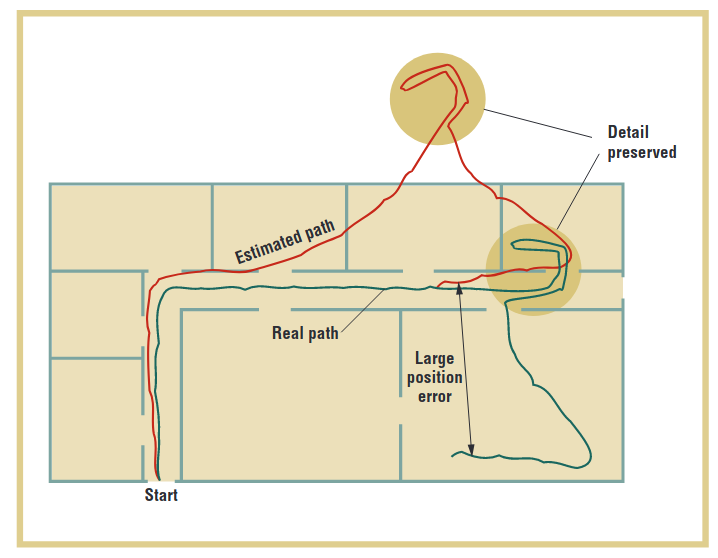
\includegraphics[width=0.8\textwidth]{figs/dead_reckoning_example.png}
    \caption{Dead reckoning example \cite{fischerLocationNavigationSupport2010}}
  \end{figure}
  \note{
    An example from an article we read where they gave an overview of different positioning techniques used for estimating firefighters' positions.\\
    Here they knew the firefighter's initial position based on where he entered the building and determines the relative position based on an inertial sensor.\\
    It can be seen that the result is not great. The issue with relative positioning is typically that the errors add up. Here it seems like the sensor got an offset error - perhaps from the firefighter looking into one of the rooms.\\
    The error can typically be corrected by a ''fix'' which in the firefighter's case is difficult but in other cases may be sensible. A sailor can re-determine the ship's absolute position if the sailor has a map with landmarks. This can then be used to determine the relative position so that he doesn't have to continously measure it from the map.
  }
\end{frame}

\section{Hybrid positioning}
\begin{frame}
  \frametitle{Multisensor data fusion}
  \begin{figure}
    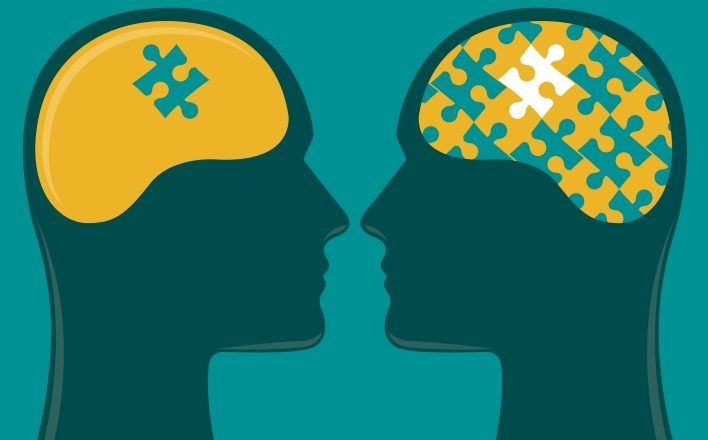
\includegraphics[width=0.6\textwidth]{figs/twoHead.jpg}
    \caption{Two heads are better than one \cite{hartPartnersInnovationWhy2014}}
  \end{figure}

  Combine relative and absolute positioning
  \note{
    Multisensor data fusion comes from the idea that if you combine the observations from multiple different sensors then you get a better outcome. ''Better'' could be more accurate, complete or dependable.\\
    If I had drawn a topic where we talk more about pervasive computing then sensor fusion could have been more interesting to talk about as an overall topic.\\
    For this topic, we can mainly use it to combine relative and absolute positioning.
  }
\end{frame}

\begin{frame}
  \frametitle{Kalman filter overview}
  Estimates noise-free signal:
  \begin{itemize}
    \item Assumes noise models are known and follow normal distribution
    \item Uses property of normal distribution
  \end{itemize}

Uses recursion:
\begin{itemize}
  \item Predict next state through a model
  \item Correct the state using measurement
\end{itemize}
\note{
  Property: The property it uses is that multiplying two gaussian distributions gives a more narrow distribution. If we consider our distributions as estimates of the true value (PDFs) then our confidence interval becomes more narrow which is great.
  
  \vspace*{2em}
  Predict: In our positioning case, this could be through relative positioning.\\
  Correct: This could be our absolute position.
}
\end{frame}

\begin{frame}
  \frametitle{Kalman overview}

  \begin{figure}
    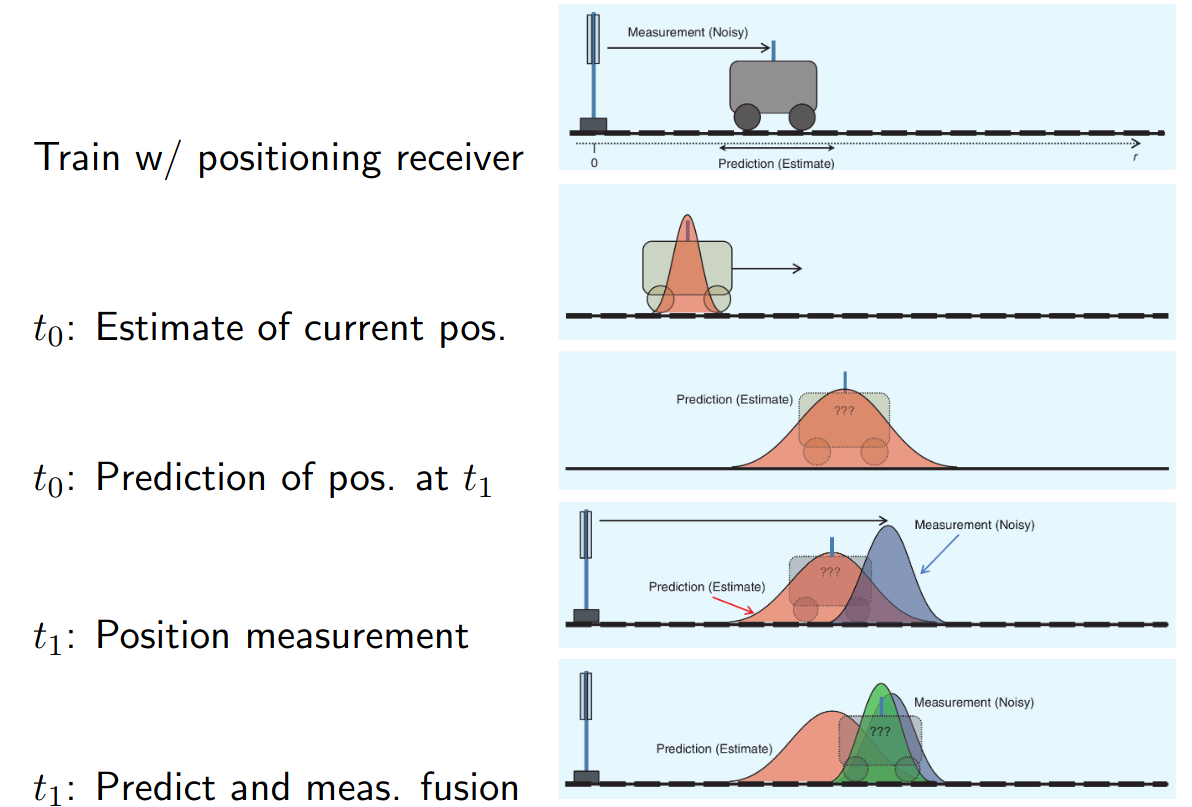
\includegraphics[width=0.9\textwidth]{figs/kalman_overview.png}
    \caption{Kalman filter explained through an example. Slide: \cite{pedersenPositioningLocationAwareness2022}. Figures: \cite{faragherUnderstandingBasisKalman2012}}
  \end{figure}
  \note{\footnotesize
    Figure 1: In this example, we have a train where we want to know the 1D position. It has a position receiver and we know the velocity.\\
    Figure 2: We have a pretty good idea of the initial position of the train at $t_0$\\
    Figure 3: Here we have been driving for a while and through dead reckoning, we want to estimate the new position at $t_1$. The difficult part here is to build a good model since with Kalman filters we need a PDF and not a single measurement. It is assumed that we know this model. Perhaps it is related to the known error of the speedometer and a function of time. The longer time we spent since the last measurement the wider the PDF.\\
    Figure 4: Now we also use our position receiver where we also model it as a PDF. The result is seen in the figure where in this case there isn't a lot of overlap.\\
    Figure 5: We combine the two PDFs which results in the green one that is more narrow. This is the model for the noise-less signal. The position we report would be the mean of the green PDF.
  }
\end{frame}

\begin{frame}
  \frametitle{Kalman filter - Result parameters}
  \begin{equation}
    PDF_{\text {fused }}\left(r ; \mu_{\text {fused }}, \sigma_{\text {fused }}\right) =\frac{1}{\sqrt{2 \pi \sigma_{\text {fused }}^{2}}} e^{-\frac{\left(r-\mu_{\text {fused }}\right)^{2}}{2 \sigma_{\text {fused }}^{2}}}
  \end{equation}
  \begin{equation}
    \begin{aligned}
    \mu_{\text {fused }} &=\frac{\mu_{1} \sigma_{2}^{2}+\mu_{2} \sigma_{1}^{2}}{\sigma_{1}^{2}+\sigma_{2}^{2}} \\
    &=\mu_{1}+\frac{\sigma_{1}^{2}\left(\mu_{2}-\mu_{1}\right)}{\sigma_{1}^{2}+\sigma_{2}^{2}}
    \end{aligned}
    \end{equation}
  \begin{equation}
      \sigma_{\text {fused }}^{2}=\frac{\sigma_{1}^{2} \sigma_{2}^{2}}{\sigma_{1}^{2}+\sigma_{2}^{2}}=\sigma_{1}^{2}-\frac{\sigma_{1}^{4}}{\sigma_{1}^{2}+\sigma_{2}^{2}}
  \end{equation}
  \note{
    I simply wanted to add this slide to show how easy it is to calculate the new PDF. The difficult part about the Kalman filter is determining the accurate models for your estimates and predictions.
  }
\end{frame}

\section{References}
\begin{frame}[allowframebreaks]{References}
  \bibliographystyle{ieeetr}
  \bibliography{references}
\end{frame}  


\begin{frame}[standout]
	Backup slides
\end{frame}

\begin{frame}
  \frametitle{Kalman filter - Prediction model}
  \begin{equation}
    \mathbf{x}_t = \mathbf{F}_t\cdot \mathbf{x}_{t-1} + \mathbf{B}_t\cdot \mathbf{u}_t + \mathbf{w}_t
  \end{equation}
  \begin{table}
    \begin{tabular}{@{} lr @{}}
      \toprule
      $\mathbf{x}_t$: & State vector. E.g. position, velocity, etc. \\
      $\mathbf{F}_t$: & State transition matrix. Applies effects of $\textbf{x}_{t-1}$ on $\textbf{x}_t$\\
      $\mathbf{u}_t$: & Control vector. E.g. braking force from driver braking.\\
      $\mathbf{B}_t$: & Control input matrix. Applies effects of $\textbf{u}_{t}$ on $\textbf{x}_t$\\
      $\mathbf{w}_t$: & Normal distributed noise model for $x_t$. $\;PDF(\mathbf{w}_t) \sim \mathcal{N}(0,\mathbf{Q}_t)$.\\ 
      $\mathbf{Q}_t$: & Covariance matrix - must be guessed.\\
      \bottomrule
    \end{tabular}
  \end{table}
\end{frame}

\begin{frame}
  \frametitle{Kalman Filter - Measurement Model}
  \begin{equation}
    \mathbf{z}_t = \mathbf{H}_t\cdot \mathbf{x}_{t} + \mathbf{v}_t
  \end{equation}
  \begin{table}
    \begin{tabular}{@{} lr @{}}
      \toprule
      $\mathbf{z}_t$: & Measurement vector. E.g. position, velocity, etc. \\
      $\mathbf{x}_t$: & State vector. E.g. position, velocity, etc. \\
      $\mathbf{H}_t$: & State-domain to measurement-domain transformation matrix.\\
      $\mathbf{w}_t$: & Normal distributed noise model for $\mathbf{z}_t$. $\;PDF(\mathbf{v}_t) \sim \mathcal{N}(0,\mathbf{R}_t)$.\\ 
      $\mathbf{R}_t$: & Covariance matrix - can be measured.\\
      \bottomrule
    \end{tabular}
  \end{table}
\end{frame}

\begin{frame}
  \frametitle{Kalman filter - recursiveness}

  \begin{figure}
    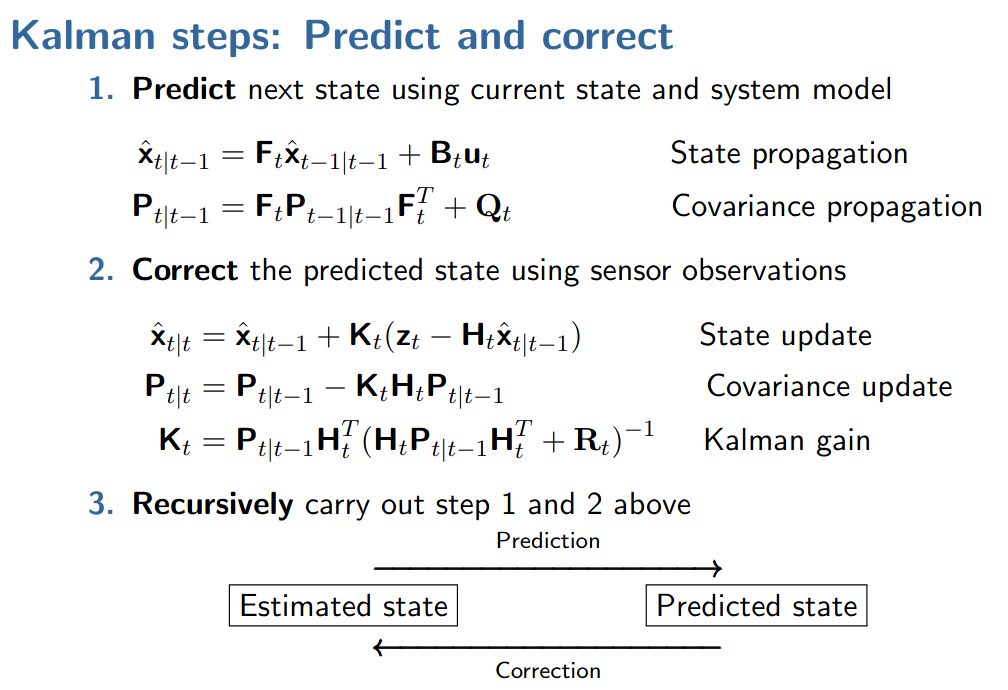
\includegraphics[width=\textwidth]{figs/kalman_recursiveness.png}
    \caption{Kalman filter \cite{pedersenPositioningLocationAwareness2022}}
  \end{figure}

\end{frame}


\end{document}
